\chapter{先行研究}
\label{chap:search}

 睡眠の研究は近年注目を浴びている。睡眠に関連する研究の中の多くはbeddit\cite{beddit}、Bed Prssure MatやiSleep\cite{iSleep}などのように睡眠のモニタリングに関連したものである。一方本研究で開発をしたスマートフォンアプリMemoryDreamは、睡眠中に人が夢を見る習慣を利用して拡張現実の体験を促すために製作された。\\
 本章では睡眠のモニタリングを目的として製作された製品と、明晰夢を促進するデバイスにおいての先行事例・研究を紹介し、さらに複数の観点からMemoryDreamとの比較を行う。

\section{モニタリング}
 MemoryDreamは睡眠中に拡張現実を体験するための手段として考えられた研究である。よって正確に睡眠をモニタリングする方法を探究するというのはこの論文の主旨ではない。しかし明晰夢に影響を与えるのに夢をみる時間帯であるREM(Rapid Eye Movement)睡眠を観測することは重要な鍵となる。以下はモニタリングに注目した先行研究である。
%ここについてもっと説明する!

\subsection{beddit}
\begin{itemize}
\item 概要:マットの上にセンサーを配置、体動を観測。睡眠の質を向上させるためにセンサーで情報を蓄積、アプリでユーザーに情報を共有。
\item モニタリング手法:鼓動によって起きる血流の変化と呼吸に伴う肺の動きをセンサーで観測。\cite{beddit}
\item 特徴:ウェラブルデバイズではないためユーザーが使用しやすいが、1,8966円のデバイスを買わなければならないのでユーザーの負担になりやすい。
%\item 正確性:46人を対象に実験し、心電計と比べた結果bedditの結果が99.94%の相関性があると証明されている
%\item 値段:18966円
\end{itemize}

\subsection{オムロン睡眠計}
\begin{itemize}
\item 概要:枕元に置くだけで電波センサーが 睡眠時間を測定。測定結果がスマートフォンに転送されて、アプリを通して、睡眠の質(寝返りの回数など)や時間を一週間単位で分析。ユーザーに適した睡眠効率向上のアドバイスをする。
\item モニタリング手法:電波センサー\cite{omron}
\item 特徴:脳波を含んでいるということで正確性が高い
:プロダクト自体デザインやアプリのユーザーインタフェースへのこだわりが評価され2012年に『グッドデザイン賞』を受賞している。
%\item 正確性:商業目的の製品のため詳しいデーターは明かされていない
%\item 値段:3630円
\end{itemize}

\begin{figure}[htbp]
\begin{center}
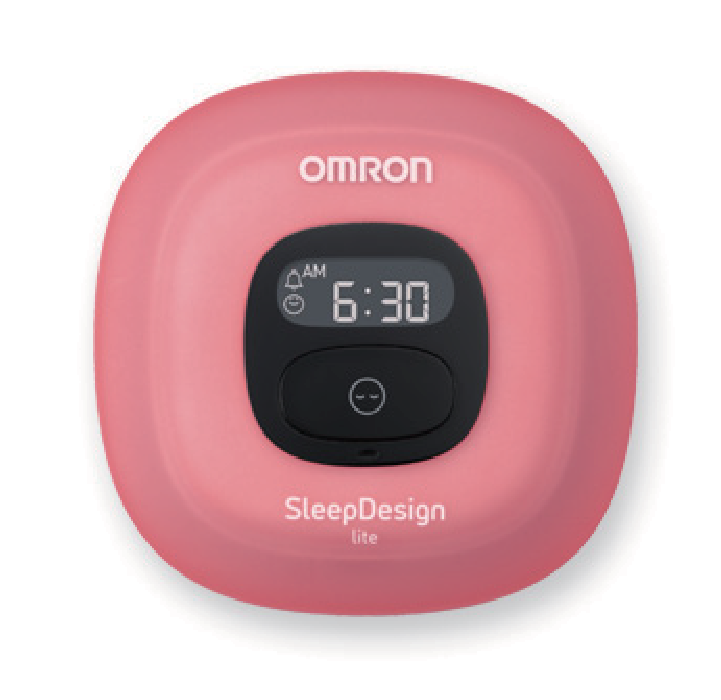
\includegraphics[width=7cm]{eps/omuron.eps}
\caption{オムロン睡眠計}
\label{omuron}
\end{center}
\end{figure}

\subsection{NEUROON TECHNOLOGY}
\begin{itemize}
\item 概要:睡眠サイクルの改善、光セラピーのためのウェラブルマスク
モニタリング手法:脳波、眼球の動き、心拍数、血液中の酸素量、加速度、体動と体温 \cite{neuroon}
\item 特徴:脳波を含んでいるということで正確性が高い。
%\item 正確性:商業目的の製品のため詳しいデーターは明かされていない
%\item 値段:36478円
\end{itemize}

\subsection{Zero}
\begin{itemize}
\item 概要:睡眠時無呼吸症候群の解決などを目的としたウェラブルデバイス \cite{beWellApp}。
\item モニタリング方法:脳波
\item 特徴:睡眠の各ステージを正確に突き止めることができ、正確性は高い。しかし頭に装着しなければならないデバイスなので汗をかきやすくなり、ユーザーの負担になるので長期的な利用には向いていない。また、寝るときにアプリに伝えないといけないので生活パターンを変えなければならない可能性がある。
%\item 正確性:睡眠のモニタリング方法としてもっとも正確とされている
%\item 値段:商業用目的ではないため不明
\end{itemize}

\subsection{iSleep}
\begin{itemize}
\item 概要:健康向上のために睡眠時間とその質をスマートフォンのアプリで観測。
\item モニタリング手法:スマートフォンに備わっている音声録音機能で体動、咳やいびきなどを測定。 \cite{iSleep}
\item 特徴:アプリをダウンロードするだけで簡単に使える。ローンチ10日間で100人のユーザーから睡眠に関する詳細なデータを集めている。
%\item 値段:361円
%\item 正確性:被験者7人51日間の睡眠で90\%の正確性
\end{itemize}

\subsection{Be Well App}
\begin{itemize}
\item 概要:うつ病、心配性、不眠症、高血圧になりにくい生活習慣へと導くために睡眠の長さを測る。
\item モニタリング手法:ユーザーによるインプットは一切必要なく、ユーザーの充電、加速度からスマートフォン利用頻度・時間を測定、静けさ、部屋の明るさなどから、睡眠スタイルを検知する。\cite{beWellApp}
\item 特徴:アプリという形で多くの人に実験をしてもらえる、ユーザーは普段の生活となんら変わりなく、過ごせるため、負担がかからない。
%\item 効果:8人の被験者に、Jawbone、Zeoと、BESモデルのアプリを試してもらい、全ての人がユーザー体験を過ごせたと結果がきた。
%\item 正確性:睡眠時間+-42分
%\item 値段:商業用目的ではないため不明
\end{itemize}

以上の先行研究を踏まえると、睡眠の感知の仕方は様々であるということがわかる。最も正確であるとされているのは眼球の動きをトラッキングする手法と脳波センサーであるが、これでは身につけるタイプのセンサーなのでユーザーの負担になってしまう。またデバイスを購入するためのコストがかかってしまうので、本論文の主旨とずれてしまうことになる。次に体動検知のために使われる電波センサーであるが、これもデバイスの購入を必要とする。そこでもっともユーザーの負担ならずに正確性も証明されているのがiSleepをはじめとするスマートフォンアプリケーションだ。こられの理由からスマートフォンアプリケーションが問題解決の手段としてもっとも適していると判断した。そこでiSleepで紹介されているアルゴリズムを参考にしたプログラムを製作した。

\section{睡眠に対するインプット}
 外的刺激を与えることで睡眠に影響を与えようとした研究や製品開発は前例がある。首都大学の長塚麻美らによる研究では睡眠深度に即した光の刺激を与える抱き枕型のインタフェースを提案している\cite{sleepSheep}。寝付きやすくするために赤に近い黄色の光を点灯させ、波の音を再生するというシステムであるが、その実験結果は明らかにされていないため評価するためにはさらに実験が求められる。
 株式会社タカラが開発した夢見工房は音、香り、視覚的情報により夢をより理想的なものに近づけるデバイスである。具体的にはユーザーが寝る前に「恋愛」、「勇気」や、「冒険」からみたい夢のテーマを選び、睡眠時にそれに紐ずいた音楽と香りが発生する。またボイスレコーダー機能もついており、みたい夢を暗示する声が目覚めない程度の小さな音量で自動的にリピート再生させることもできる。 \cite{takaratomi}このように多くの機能が備わっており、気分転換や充実した楽しい時間を作り出すことを目的としているが、正式な効果は発表されていない。また香りや音声の種類に限りがあるというも、問題である。値段も14,800円と高めである。
\begin{figure}[htbp]
\begin{center}
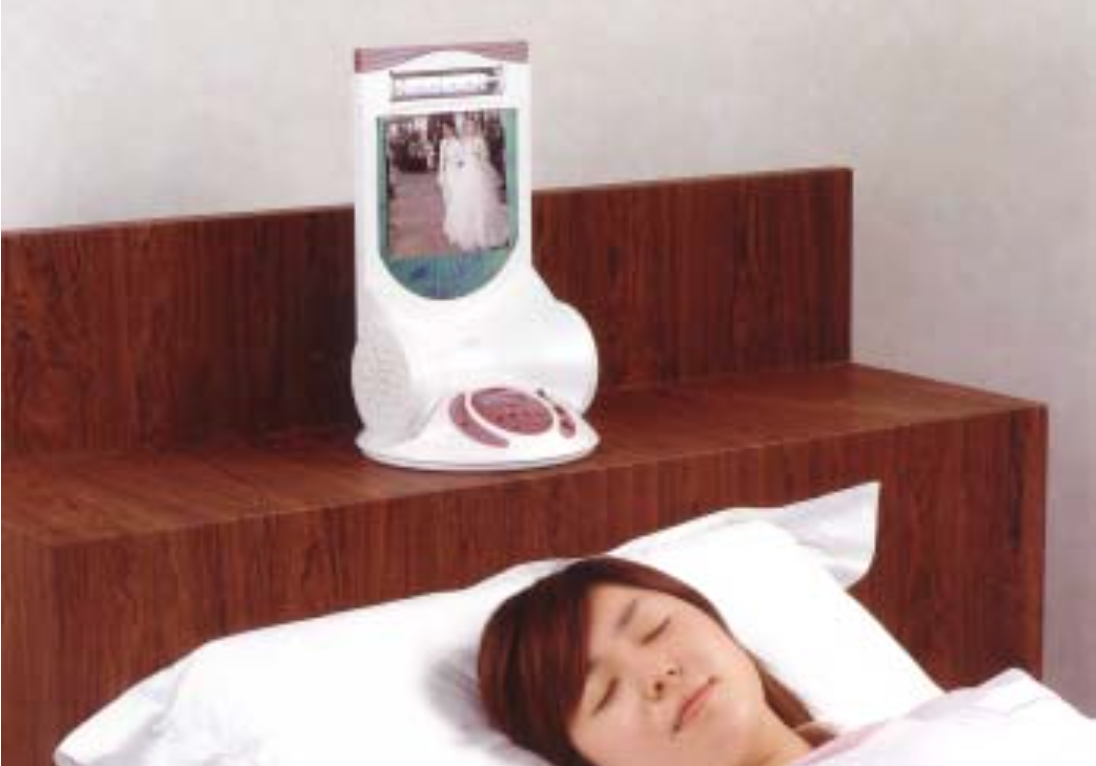
\includegraphics[width=10cm]{eps/takaratomi.eps}
\caption{夢見工房のイメージ}
\label{takaratomi}
\end{center}
\end{figure}

 他にも明晰夢を促進するとためのツールとしてiWinksにより開発されたAURORAがある。\cite{iWinks}これはREM睡眠時に光による刺激を与えることで、ユーザーに夢を見始るという暗号を送って明晰夢を促すデバイスである。脳波センサー(EEGセンサー)と加速度センサーが組み込まれており、睡眠の質観測においてはクリニックにより検証されたものとウェブページ上には書かれている。しかし明晰夢への効果に関する実験結果が明らかになっていないので、真実であるという確証はない。値段も3,6000円と非常に高額である。
 他にもDreamOnというスマートフォンアプリがある。睡眠中に音楽を流すことで夢に影響を与えるアプリだ。アプリという形で多くの人に夢の研究に参加してもらい音が夢に影響を与えるのか否かについて判明することを目的としている。 \cite{dreamOn}レーティングは3であり、385のレーティングが残っている。ウェブサイトには睡眠は外的刺激に影響を受け、例えば森林の音を流すと夢の中に緑が頻繁に現れて、街中の音を流すと奇抜な夢を見ると書いてある。しかし実験結果についてはかなり疑わしい。下記の画像\ref{DreamOnImage}はユーザーのレビューである。悪夢を見たなどの睡眠被害を訴えるレビューが多く見受けられた。DreamOnの他にもユメミール \cite{yumemiru}やDreamDream \cite{DreamDream}など国内のアプリもあるが、どれも信ぴょう性のある実験結果は公開されていない。

\begin{figure}[htbp]
\begin{center}
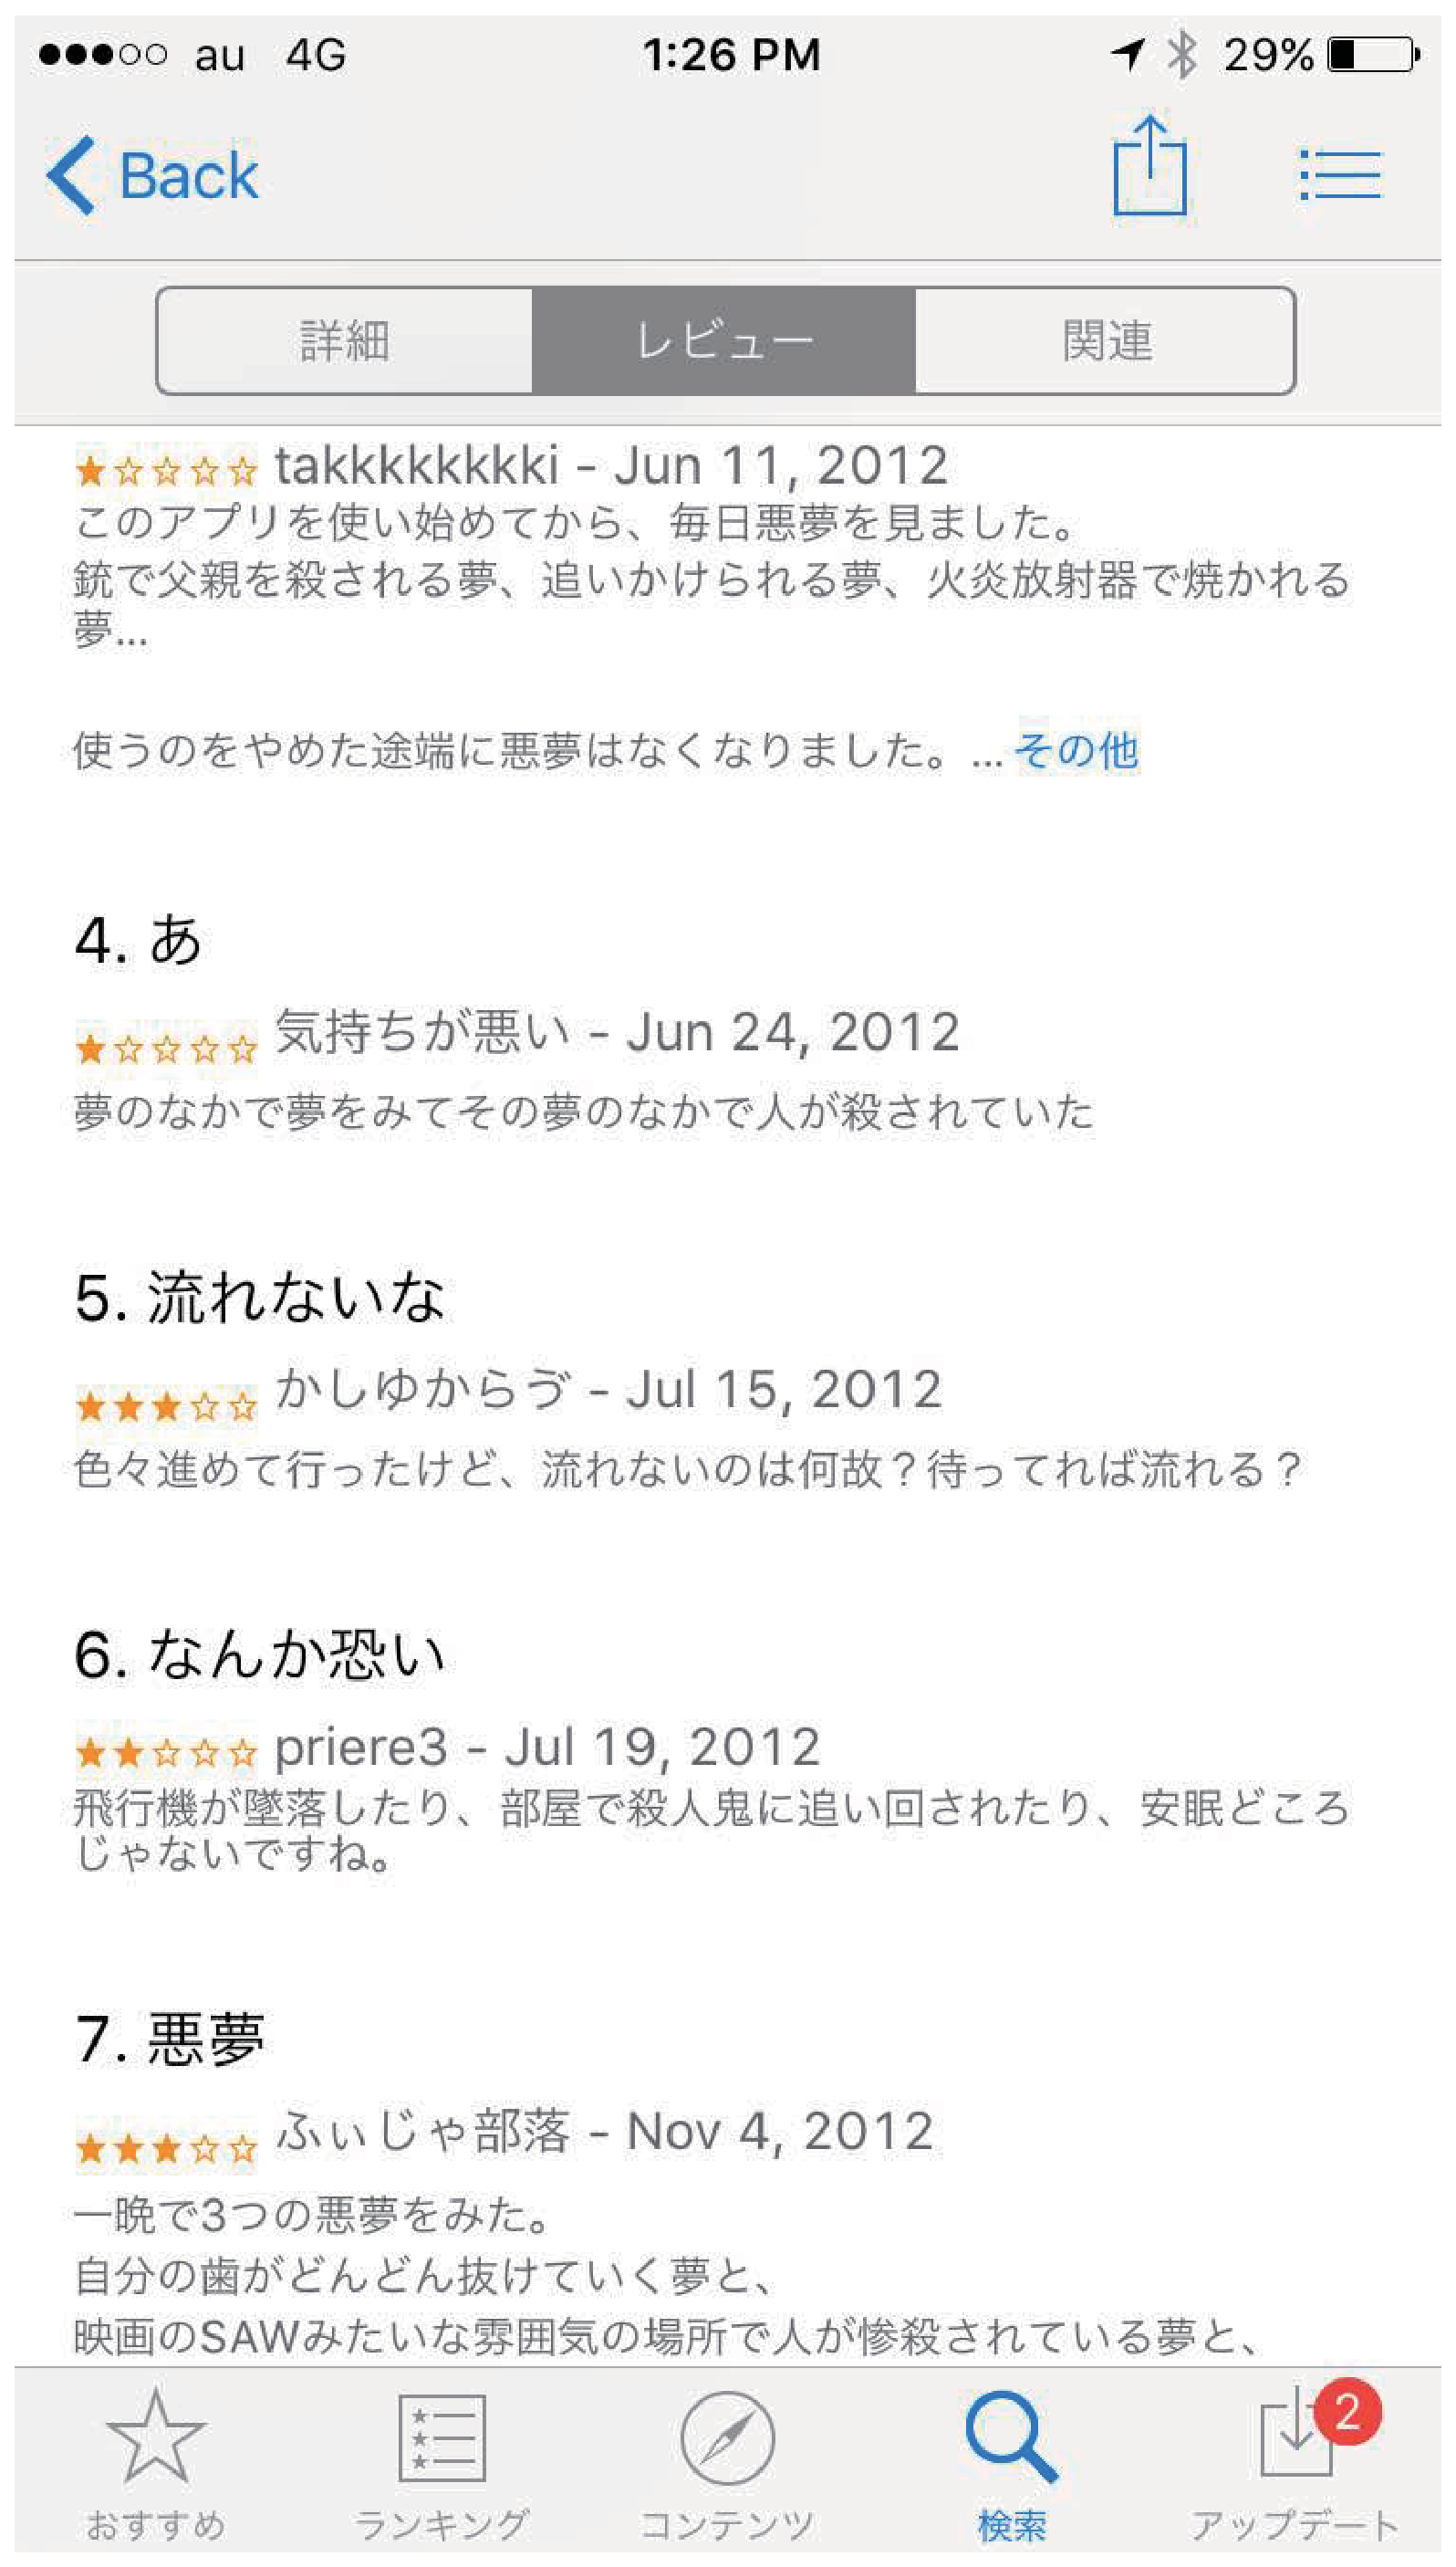
\includegraphics[width=6cm]{eps/dreamOn.eps}
\caption{DreamOnアプリのレビュー}
\label{DreamOnImage}
\end{center}
\end{figure}

\section{MemoryDreamの立ち位置}
夢を操作するために多くの研究が行われてきたが、実験結果については明らかになっていないのが現状だと思われる。これらの先行研究を参考にしてMemoryDreamは以下の点を明確にしたい。
\begin{itemize}

\item 実験内容と結果が明快かつ詳しい。
\item コストのかかるデバイスを必要としない。
%スマートフォンアプリケーションを使う。
\item ユーザーによってカスタマイズが容易であること
%音声登録が容易である。

\end{itemize}